\citeauthor{Huron2013} proposed a novel design metaphor inspired by the physical process of sedimentation. The design metaphor is called visual sedimentation and describes the process of aggregating falling objects due to gravity over time into static shapes \iacite{Huron2013}. This concept can be applied very well to streamed data. Incoming data items would be represented by falling objects, animated by virtual forces and aggregating over time in static shapes.
The basic concept of visual sedimentation can be described in four steps:

\begin{enumerate}
\item A new data item is processed and ``enters'' the scene.
\item Virtual forces are applied to the data item and suspension occurs while falling to the ground.
\item Items are accumulated on the ground or on top of previous items.
\item Items are merged into an aggregated shape.
\end{enumerate}

The possible datasets for visual sedimentation are quite obvious: all the examples discussed in the paper are some kind of dynamic, streamed data including a temporal attribute. This fact already answeres the first question of the analysis framework. Nonetheless, the concept and the examples could be extended with using static datasets without any kind of attribute of a temporal nature. Preprocessing and sorting the dataset before dropping items into the scene could yield interesting results. The weakness of using static datasets is that it stops after every item being processed. Aggregating an item into a static shape is based on multiple decisions in visual sedimentation. Thus it yields to non-aggregated data items on top of an aggregated shape when the dataset is finished. This does not happen when using streamed data.
The reason that visual sedimentation does not allow any kind of interaction leads to the answer of why even use it. It is mainly used to present some kind of data and to enjoy the visualisation itself. It is not possible to get more information on neither a single data item nor an aggregated shape.
The discussed examples are all based on two facts:
\begin{enumerate*}[label={(\arabic*)}]
\item all of them use streamed data including a temporal variable and
\item all data items have the same categorical attribute.
\end{enumerate*}
Thereby, visual sedimentation makes use of visualisations which are able to handle categorical data and use color as the visual encoding channel.

\begin{figure}[!htb]
\centering
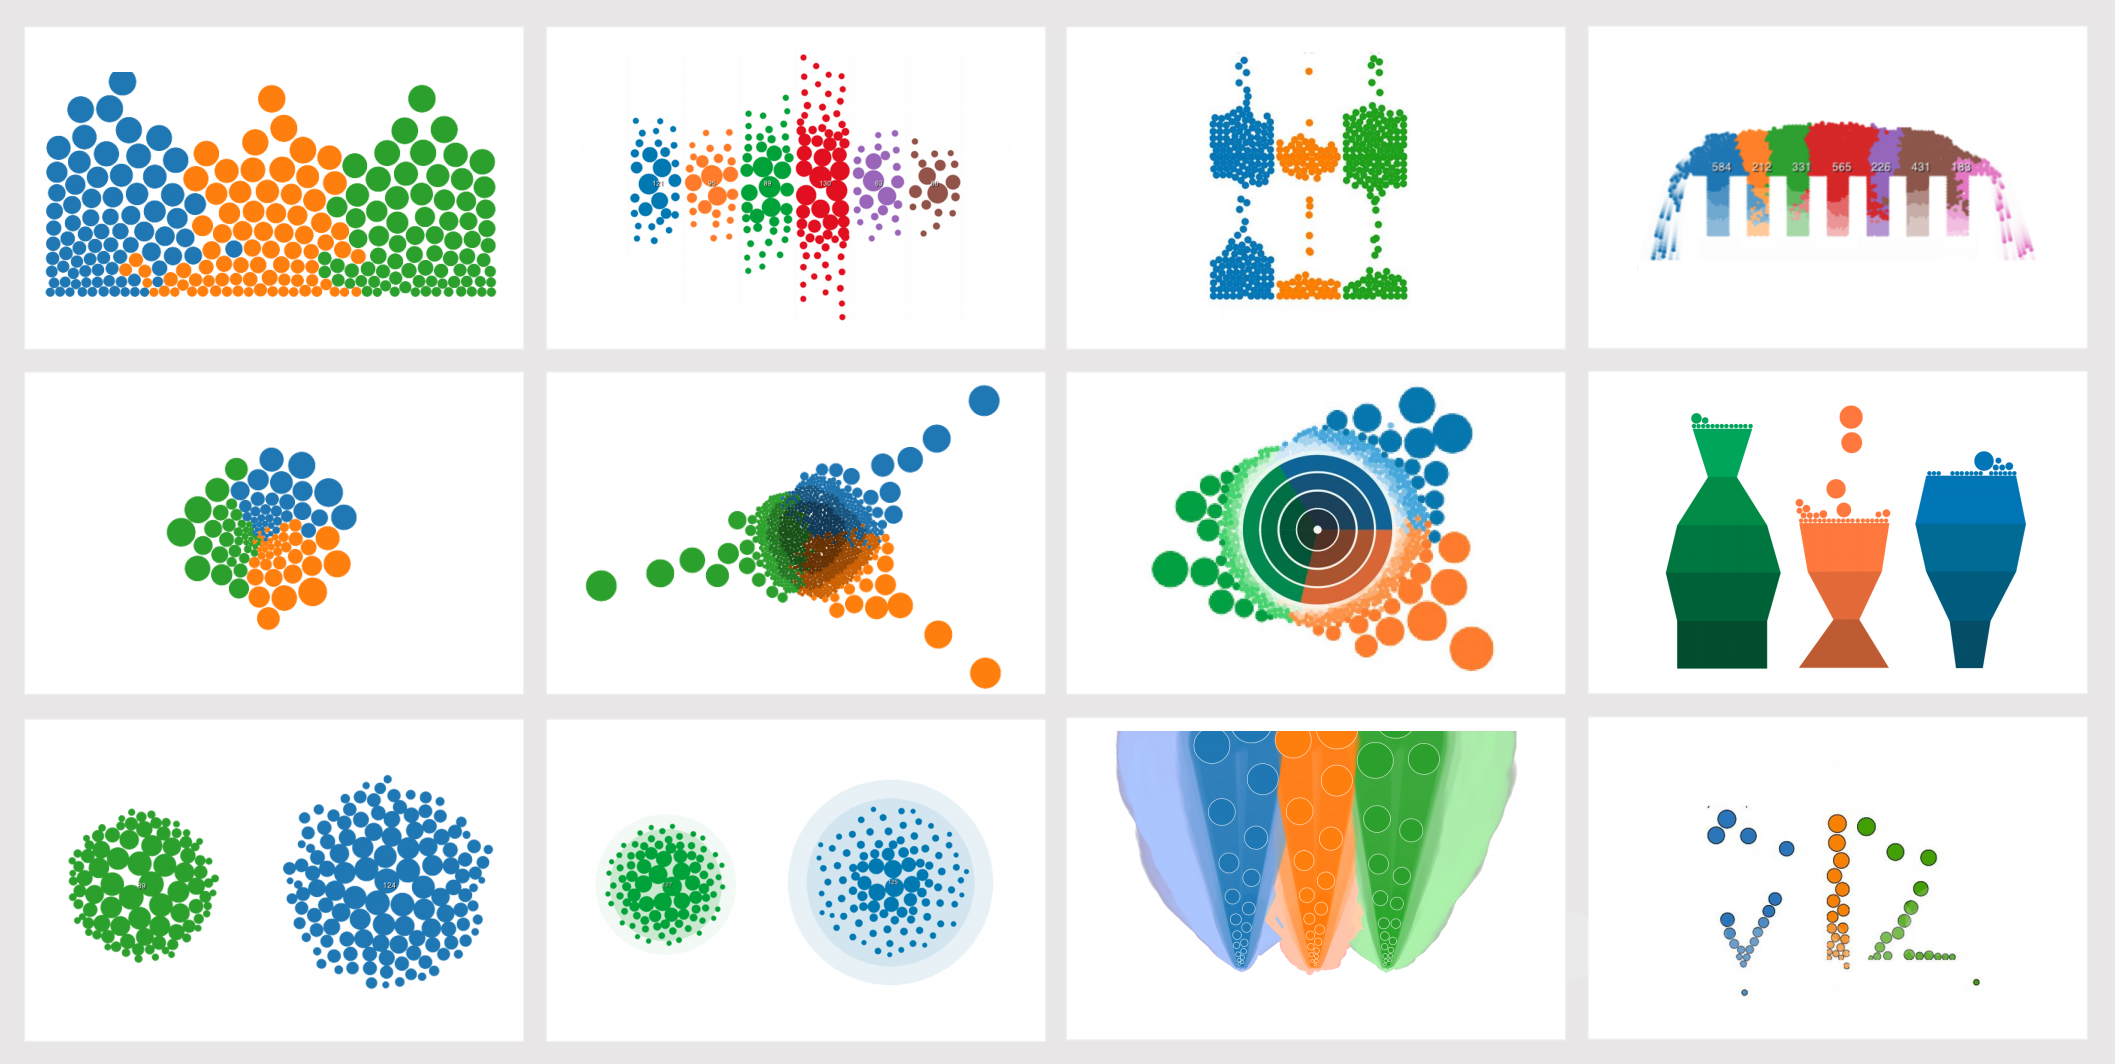
\includegraphics[height=5cm]{images/methods/related/visual-sedimentation}
\caption[
    Charts created by visual sedimentation \iacite{Huron2013}.
]{Charts created by visual sedimentation}
\label{fig:visual-sedimentation}
\end{figure}
\cbstart
Figure \ref{fig:visual-sedimentation} on page \pageref{fig:visual-sedimentation} shows possible charts made by visual sedimentation. Considering an animated transition from a visualisation type to an upcoming visualisation based on aggregation, using the concept of visual sedimentation and animating the aggregation could affect the user's comprehension of the visualisation. Being able to actually follow the creation of a visualisation could reveal its strengths and weaknesses.
\cbend